%
% Manchester Raspberry Jam Workshop Booklet
%
% This template is designed to try and aide consistency between each booklet.
% Insert files as instructed by comments, things like tables of contents are created by other linked files
%

% Enter the document title here
\newcommand{\workshopTitle}{Getting Started with Raspberry Pi}

% Enter the author of this workshop
\newcommand{\workshopAuthor}{Jack Kelly}

\input{McrRaspJam/Common/booklet_preamble}
\begin{document}
	% Title Format
\ifprint
	\title{Manchester Raspberry Jam \\ \workshopTitle}
\else
	\title{
		\begin{center}
			
\includegraphics[width=30mm]{McrRaspJam/Common/logo-512}
		\end{center}
		\vspace{12pt}
		\workshopTitle
	}
\fi

%Author (disabled until multiple authors have worked on Workshop booklets (: )
\iffalse
\author{
	Written by \workshopAuthor
	}
\fi
	
\author{}
\date{}
\maketitle

% Online download location
\ifprint
	\begin{mdframed}[rightline=false, leftline=false]
		\footnotesize
		This booklet is available online at \mbox{\href{https://drive.google.com/open?id=0B_1SFjX_5JrmfnhpX0pPRXl6bmJNal8zdUxMeWZOdjJyZVdzU3V6UnBGdlVIMENtbFFkbVk}{bit.ly/McrRaspJam}}
		\normalsize
	\end{mdframed}
\fi
	
	%
	% Input the main CONTENT below, sans title page or contents.
	% Recommend inputting per section, and adding page breaks here.
	%
	
		%Workshop Description
	The notes include a number of guides to help you get your own Raspberry Pi up and running. You should:
	
	\begin{itemize}[nosep]
		\item \textbf{Read \autoref{sec:PiEquiptment}} if you're unsure if you have everything you need to run a Raspberry Pi.
		\item \textbf{Read \autoref{sec:NOOBS}} if you want to set up a blank SD card for the Raspberry Pi.
		\item \textbf{Read \autoref{sec:setup}} to troubleshoot common problems when booting your Pi.
		\item \textbf{Read \autoref{sec:Resources}} for a collection of Raspberry Pi resource sites, where you'll find magazines, tutorials and project ideas.
	\end{itemize}
	
	\subsection*{About these booklets}
		
	%Aknowledgements
	These workshop booklets were created using {\fontfamily{rfdefault}\selectfont \LaTeX}, an advanced typesetting system that is widely used for several sorts of books, academic reports and letters.
	
	%License spiel
	To allow modification and redistribution of these booklets, they are distributed under the \hbox{CC BY-SA 4.0} License. LaTeX source documents are available at \url{http://github.com/McrRaspJam/booklet-workshops}				
	
	%File Downloads
	All of our workshop resources are available to download from a Google Drive at
\url{http://bit.ly/mcrraspjam}.
There, you can find a PDF copy of this booklet, as well as template and completed program files for each workshop.
			
	%Code Listings
	%	When you need to make changes to your code, they'll be presented in \textit{listings} like the example below. Some lines may be repeated across multiple listings, so check the line numbers to make sure you're not copying something twice.

	\lstinputlisting[style=Python, breaklines=true]{McrRaspJam/016_Ciphers/0_introduction/alphabet.py}
	
	
	
	%When you need to type a command in the command line interface, they will be listed like the following example. Copy everything \textit{after} the dollar sign. Lines without dollar signs are example outputs, and do not need to be copied.
			
\begin{lstlisting}[style=Terminal]
$ java HelloWorld
Hello, World!
\end{lstlisting}
	%Occasionally, a concept will be explained in greater detail in \textit{asides}, like the one below. You can read these as you wish, but they're not required to complete the workshop.
	
\begin{aside}[Resistors]
	Resistors are most commonly used to limit the amount of current flowing through part of an electrical circuit.
	
	For example we use resistors in series with LEDs, as otherwise they could draw so much power that they destroy themselves.
	
	Buttons have almost no internal resistance, so we use high value ($\sim 10  k\Omega$) resistors to prevent current flowing straight from the power supply to ground; if we didn't, the entire CPU could be short circuited, and the Pi would lose power!
\end{aside}
		
	\subsection*{Questions?}
		If you get stuck with any of the instructions, find errors or have feedback about these booklets, email:
		\url{jam@jackjkelly.com}\label{email}
	\section{What equipment you'll need}
\label{sec:PiEquiptment}

	The Raspberry Pi is a full personal computer on a single board, so we can think of it as a replacement for an old tower-style desktop machine.
	
	To get the Raspberry Pi working then, we need to add the same peripherals as we would with a desktop machine:
	
	\begin{itemize}[nosep]
		\item A TV/computer \textbf{monitor}, to output to.
		\item A \textbf{keyboard} and \textbf{mouse} for input.
	\end{itemize}
		
	In addition, the Raspberry Pi also requires:
	\begin{itemize}[nosep]
		\item A \textbf{Micro USB power supply}, the type used to charge most Smartphones and Tablets.
		\item An 8GB or larger \textbf{MicroSD card}.
	\end{itemize}
	
	\subsection*{Monitor}
	
		The Raspberry Pi uses HDMI for display output. Most modern TVs and monitors will have a HDMI port. You'll need a standard HDMI cable to connect them.
		
		\begin{figure}[h]
			\centering
			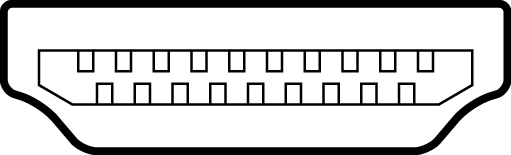
\includegraphics[height=22pt]{McrRaspJam/000_IntroToPi/1_EquipmentNeeded/HDMI}
			\\A HDMI connector
		\end{figure}
		
		If you're using a computer monitor that is a few years old, it may only have a DVI port. In this case, you can use a DVI-HDMI cable to connect to the Raspberry Pi, which can be cheaply purchased.
	
		\begin{figure}[h]
			\centering
			
\includegraphics[height=22pt]{McrRaspJam/000_IntroToPi/1_EquipmentNeeded/DVI}
			\\A typical DVI connector
		\end{figure}
		
		If possible, avoid using VGA connections. They require an (expensive) active adaptor, and are an analogue connector, so produce poorer image quality.
		
		\begin{figure}[h]
			\centering
			
\includegraphics[height=22pt]{McrRaspJam/000_IntroToPi/1_EquipmentNeeded/VGA}
			\\A VGA connector
		\end{figure}

	\subsection*{Keyboard and mouse}
	
		You can use any standard USB keyboard and mouse.
		
		The Linux Operating System that the Raspberry Pi runs also has great compatibility with most wireless peripherals that use a USB dongle, or for Pi 3 the built-in Bluetooth.
		
	\subsection*{Power Supply}
	
		Most phone chargers will boot a Pi, but if you're using add-on boards or multiple USB peripherals, you may run into power issues.
		
		Check the rating on your power supply, \url{raspberrypi.org} recommends an output rating of 5V 1.2A for a Gen1 Pi, and 5V 2.5A for a Pi 3.
		
	\subsection*{MicroSD Card}
	
		The Raspberry Pi does not have a built in ``Hard drive'' like a desktop tower, so the operating system and files are all stored on a MicroSD card.
		
		Your card will need to be \textbf{at least 8GB}, and is recommended to have a speed class of SDHC \textbf{class 10}, denoted by either the ``C10'' logo or a ``U'' logo of any number.
	
		\begin{figure}[h]
			\centering
			
\includegraphics[height=22pt]{McrRaspJam/000_IntroToPi/1_EquipmentNeeded/SDclass10}
			\hspace{12pt}
			
\includegraphics[height=22pt]{McrRaspJam/000_IntroToPi/1_EquipmentNeeded/UHSclass}
			\\SDHC Class 10 \& UHS Class 1
		\end{figure}
		\newpage
	\section{Installing NOOBS}
\label{sec:NOOBS}

	On most Raspberry Pis, we usually run an operating system called Raspbian, which is a variant of the GNU/Linux operating system.
	
%	\begin{aside}
%		Because the ARM processor in the Raspberry Pi is similar those found in billions of smartphones around the world, there are lots of other operating systems to choose from, such as other Linux distributions like Ubuntu or Arch, mobile OS's such as Android, and even a variant of Windows 10.
%	\end{aside}
	
	Raspbian can be quite tricky to install on an SD card, so a piece of software called NOOBS is provided to do most of the work for us.
	
	Many Raspberry Pi retailers sell SD cards with NOOBS pre-installed, but if you have chosen to use or purchase a blank MicroSD card, installing NOOBS yourself is straightforward.

	\subsection{Download and Install}
	
	The following instructions are for Windows 10, but should be fairly similar to most operating systems, including other versions of Windows, and MacOS.
		
	
		\begin{enumerate}[nosep]
			\item \textbf{Format your MicroSD card as a FAT file system.}
			
			On windows, right click on the SD card in the file explorer, and click `Format...'.	Most settings can be left as normal, ensure the file systems is set to `FAT32', then press Start.
			
			\begin{center}
				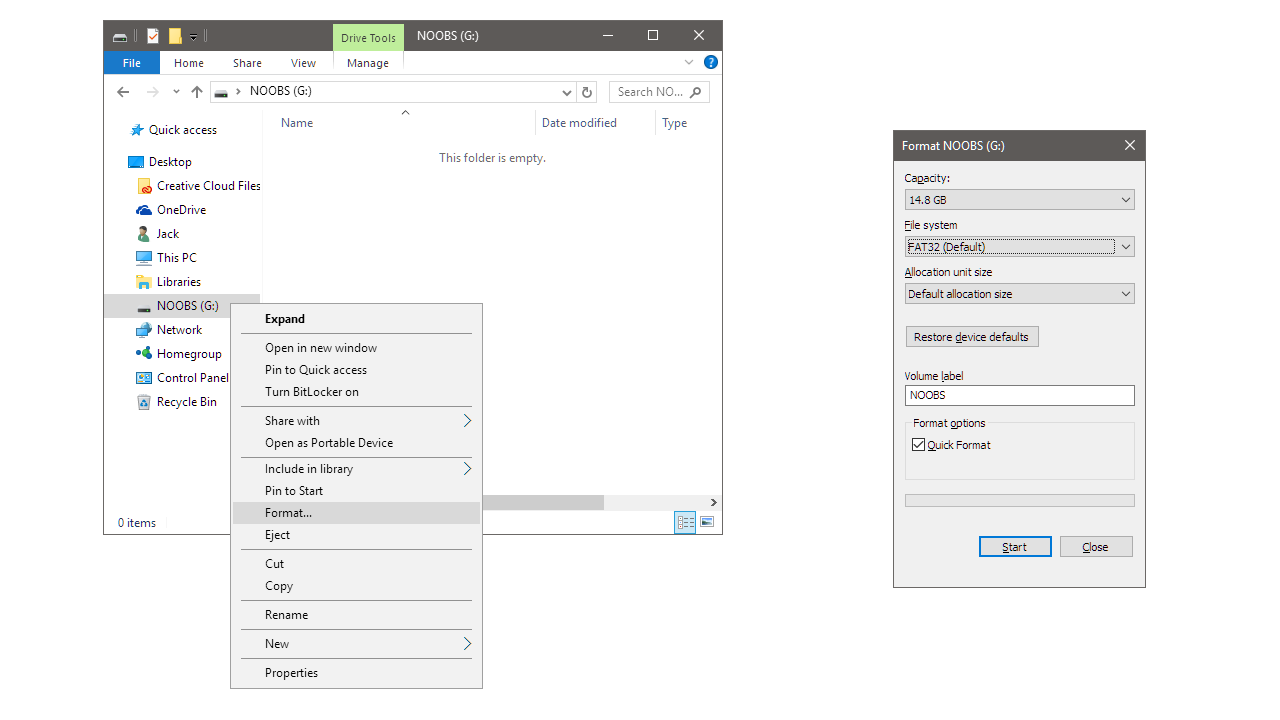
\includegraphics[width=1\linewidth]{McrRaspJam/000_IntroToPi/2_NOOBS/noobs2}
			\end{center}
			
			\item \textbf{Download the latest version of NOOBS} from \url{https://www.raspberrypi.org/downloads/}
			
			Click the `Download ZIP' button of NOOBS on the following page.
			
			\begin{center}
				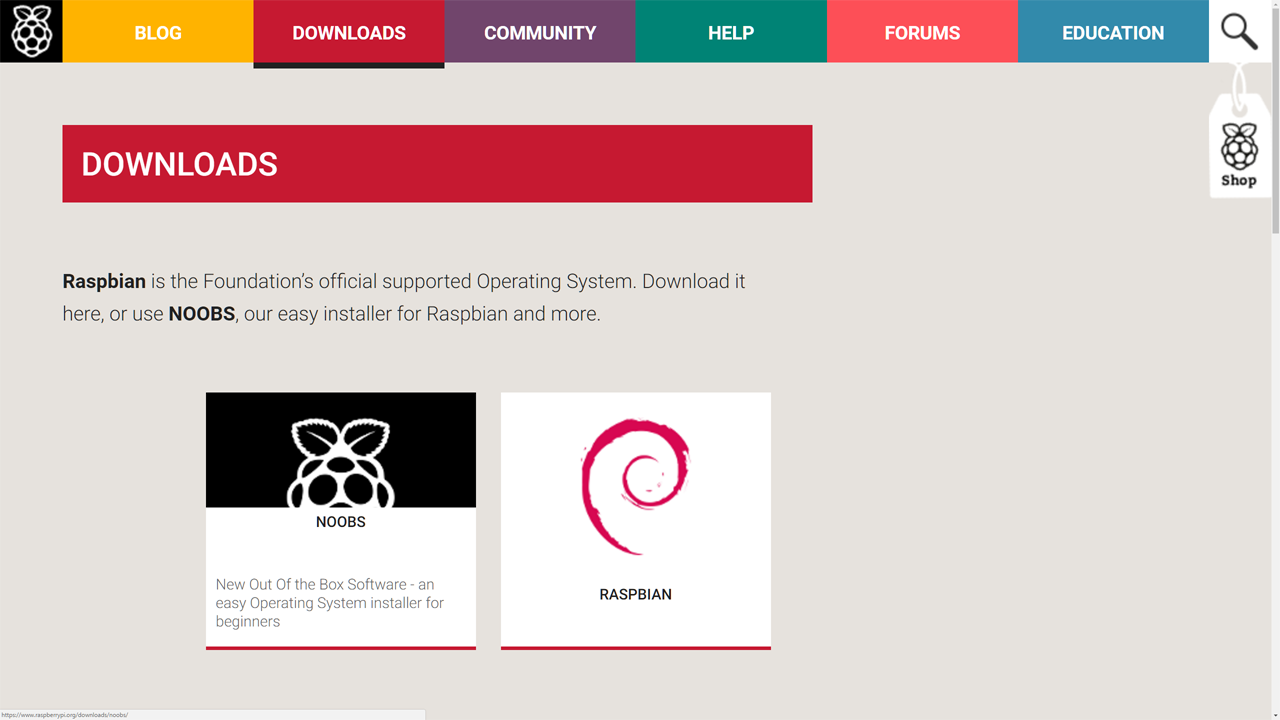
\includegraphics[width=0.8\linewidth]{McrRaspJam/000_IntroToPi/2_NOOBS/noobs1}
			\end{center}
			
			\item \textbf{Extract the downloaded NOOBS ZIP file onto the SD card}.
			
			On windows, you can right click and `Extract All...' to the drive letter of your SD card e.g. `G:\textbackslash'.
			
			\begin{center}
				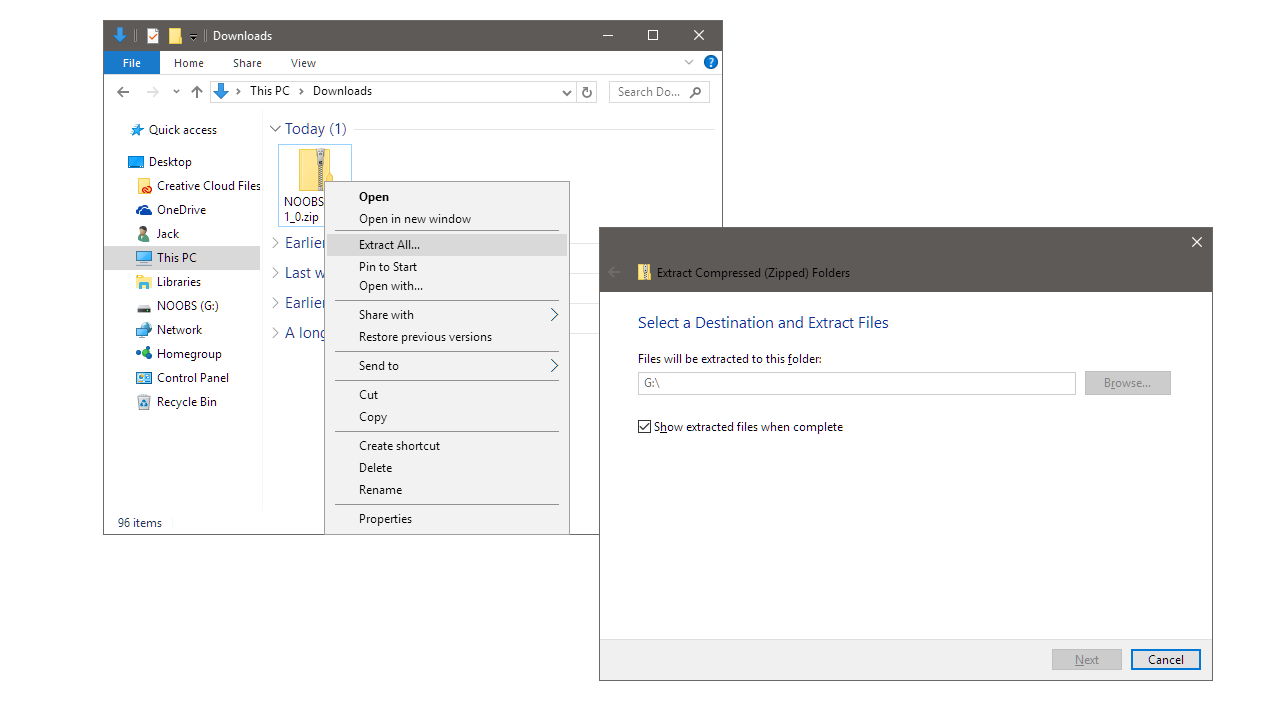
\includegraphics[width=1\linewidth]{McrRaspJam/000_IntroToPi/2_NOOBS/noobs3}
			\end{center}
		\end{enumerate}
		
		Ensure the files are extracted to the top level of the SD card, and not inside a subfolder.
		
		\subsection{Booting and Installing Raspbian}
		
		Once you have a NOOBs card set up, you can boot your Pi with it. You should see a screen like the following.
		
		\begin{center}
			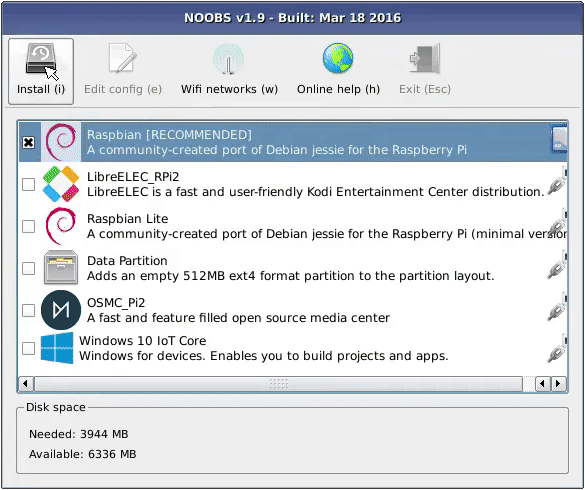
\includegraphics[width=0.8\linewidth]{McrRaspJam/000_IntroToPi/2_NOOBS/noobs5}
		\end{center}
		
		Select Raspbian (which is the only option when offline) and click install. Follow through any prompts until you reach a loading screen.
		
		The rest of the process is automatic -- and very slow -- so now is the time to find something to do for the next 20 minutes!
		
		
	

		\newpage
	\section{Booting the Pi}
\label{sec:setup}

	When booting the Pi, you should insert all of the connectors and the MicroSD card first, then insert the Micro USB power \textbf{last}, as this will cause the Pi to boot.
	
	If all goes well, the Pi should boot automatically. If not, here are some tips on spotting problems with your connections and equipment.
	
	\subsection*{Power Issues}
		
		The tell-tale sign for power issues is that the Pi will get at least partway through the boot process, then reset to the beginning.
		
		If nothing appears on the monitor, check other possible causes first.
		
	\subsection*{Display Issues}
	
		Monitors tend to be fiddly when picking up new input sources. For a sanity check it's a good idea to have another device that outputs HDMI so you can test the monitor is working, such as a laptop.
		
		If your test device outputs correctly but your Pi does not, it is likely to be an SD card issue.
		
	\subsection*{SD Card Issues}
	
		If there is an issue with your SD card, the Pi will usually not boot at all. The best way to spot this is to watch the green CPU activity light on the Raspberry Pi board. During a normal boot this will flash on and off, so if it's stuck on, the SD card is likely faulty.
	
		SD card issues can usually be fixed by formatting and reinstalling NOOBS. Use the official SD formatter tool from \url{https://www.sdcard.org/downloads/} to format your card if your OS's built in formatter did not work.
		
		A small number of SD Cards do not work with the Raspberry Pi. A compatibility list of SD cards is maintained at \url{http://elinux.org/RPi_SD_cards}, though it is not exhaustive.
		\newpage
	\section{Tutorial Resources}
\label{sec:Resources}

	Below are some top sources guides and tutorials for the Raspberry Pi 
	
	\subsection{Raspberry Pi Tutorials}
	
		\subsubsection*{Raspberry Pi Resources}
	
			\url{https://www.raspberrypi.org/resources/}
			\begin{center}
				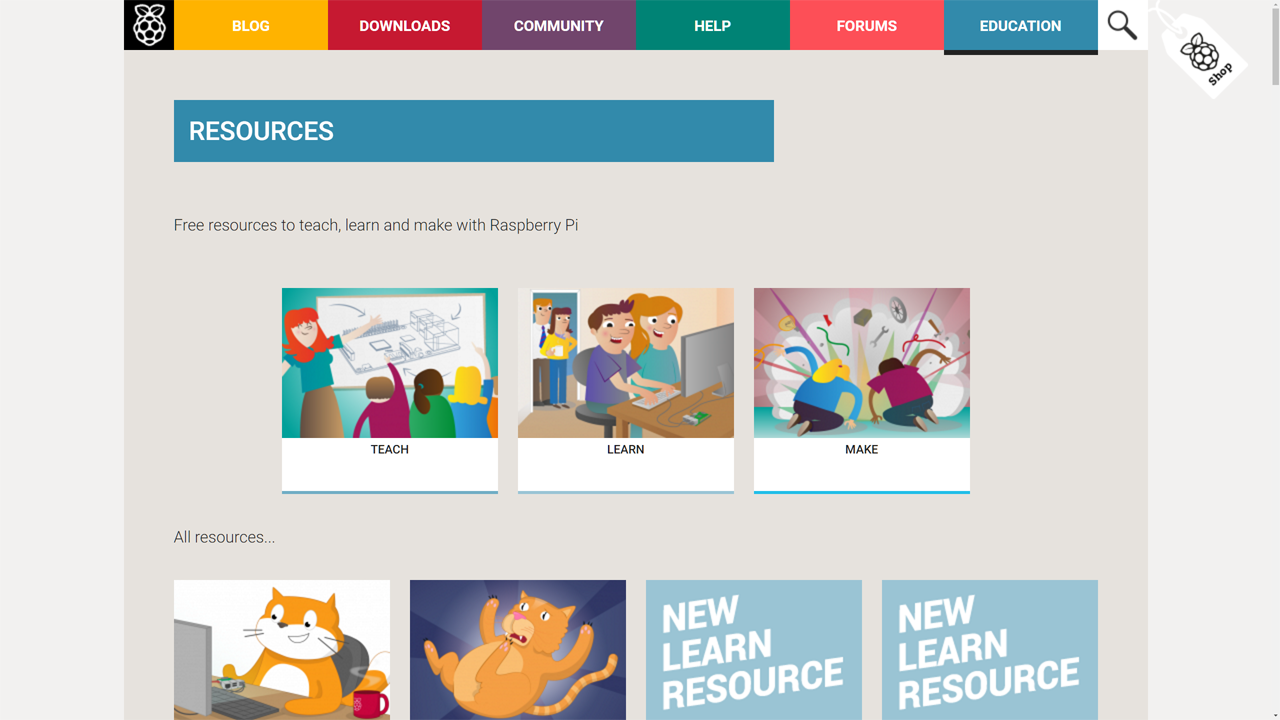
\includegraphics[width=0.5\linewidth]{McrRaspJam/000_IntroToPi/4_Resources/raspberrypiorg}
			\end{center}

	
			The official Raspberry Pi website should be your first stop, it's chock full of introduction tutorials and project ideas for most of the software we've covered today.
	
		\subsubsection*{The MagPi Magazine}
	
			\url{https://www.raspberrypi.org/magpi/}
			\begin{center}
				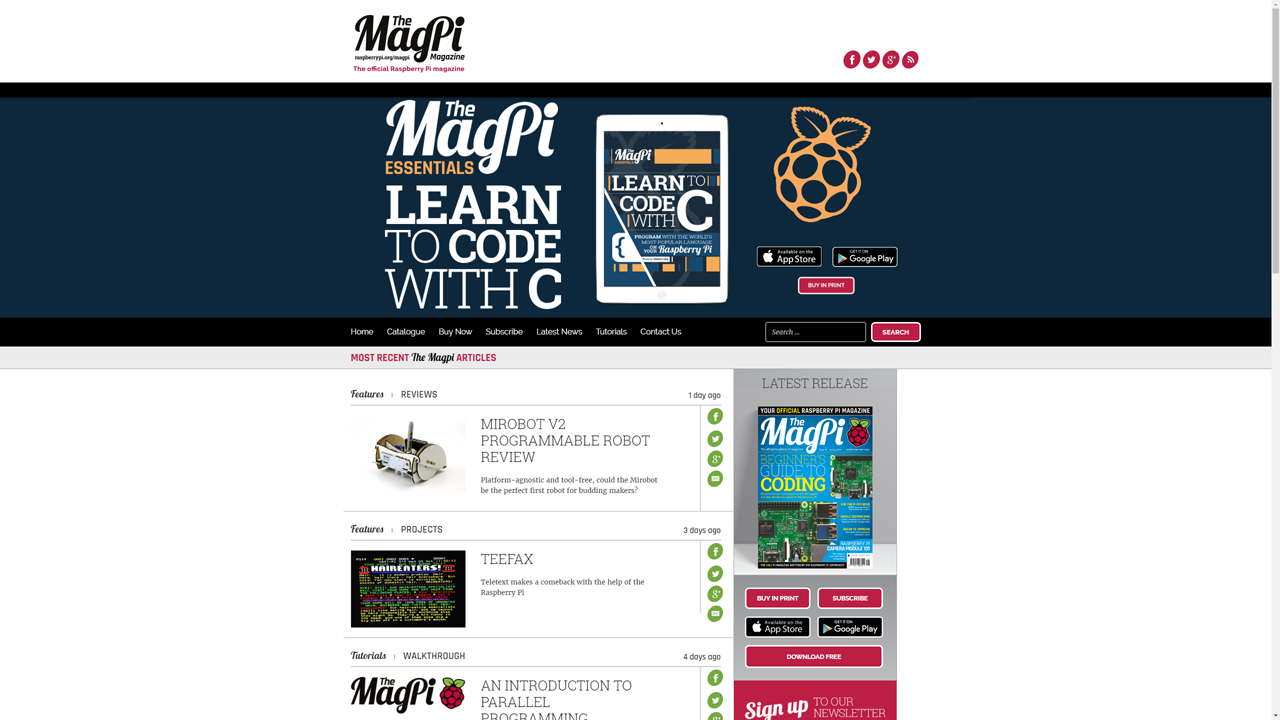
\includegraphics[width=0.5\linewidth]{McrRaspJam/000_IntroToPi/4_Resources/magpi}
			\end{center}		
				
			The MagPi started as a community run print magazine for the Raspberry Pi, and has now become the official magazine of the Raspberry Pi.
			
			Available in print (can be found in many supermarkets), or as a free download, each one is filled with articles, features and tutorials, all for the Raspberry Pi.
			
		\subsubsection*{The Raspberry Pi Guy}
			
			\url{http://www.theraspberrypiguy.com/tutorials/}
			\begin{center}
				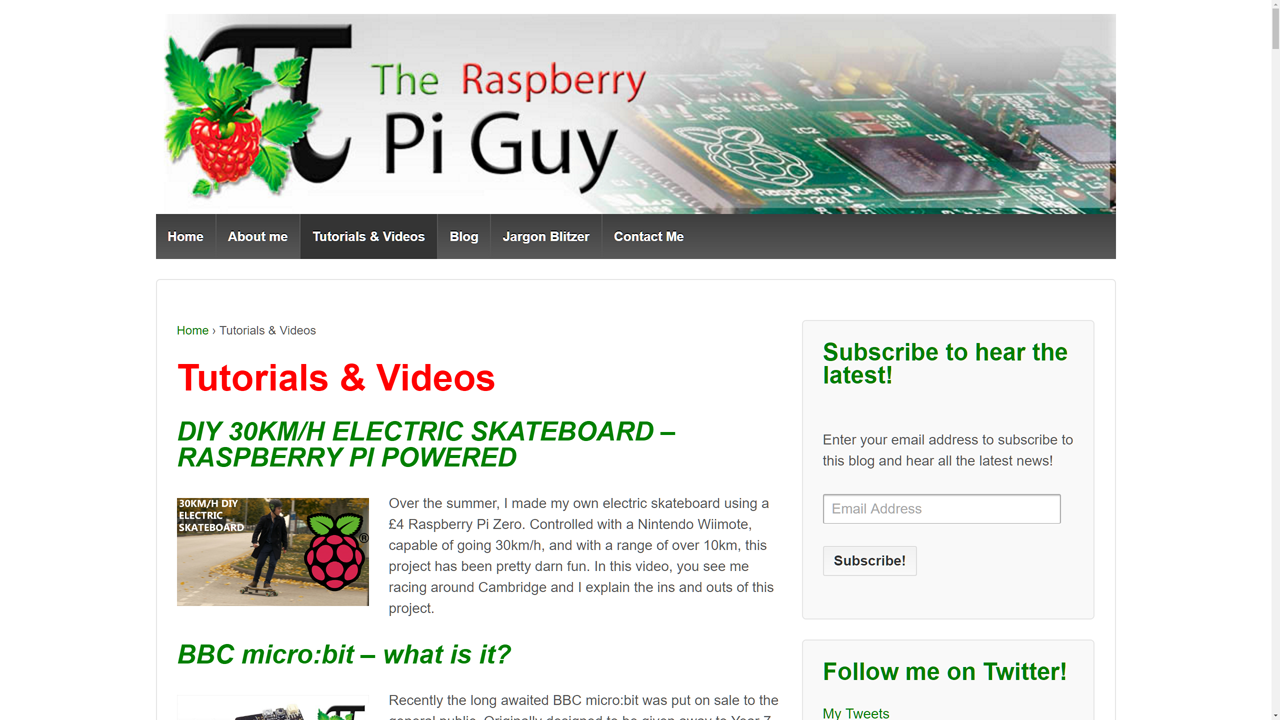
\includegraphics[width=0.5\linewidth]{McrRaspJam/000_IntroToPi/4_Resources/piguy}
			\end{center}	
			
			Matt was one of the first people to start producing regular video content for the Raspberry Pi, he was only 12 when the Pi was first released!
			
			Every few months, he produces a new video tutorial, showing off cool projects and uses for the Raspberry Pi, covering things as wide as Steam game streaming, robotics, or even building an electric skateboard.
		
	\subsection{Programming Language Tutorials}
	
		Ready to stretch your legs and try another programming language? Here are some places to look for quality programming language tutorials
		
		\subsection*{Codeacademy}
		
		\url{https://www.codecademy.com/}
		
		Codeacademy has tutorials for a large number of languages, we'd recommend \textbf{Java} for a great second language and introduction to object orientated programming, or \textbf{Javascript} if you'd like to learn some programming for web purposes. Confusingly, Java and Javascript are entirely seperate languages.
		
		\footnotesize \textit{Codeacademy offers paid features like multiple-choice quizzes, but these aren't necessary to learn the language, and none of the core content is paywalled.} \normalsize
	
		\subsection*{C and C++}
		
		\url{http://www.learn-c.org/}
		\\ \url{http://www.learncpp.com/}
		
		If you're feeling brave, C and C++ are traditional programming languages that are widely used today. C++ was designed to follow on from C, so it makes sense to start with C.

\end{document}